\section{包含映射}
\label{sec:lop-inclusions}

一个函数可以同时属于几个函数空间，并在各自的范数下得到不同的“大小”。若我们在一个空间的范数下估计了误差，常常还想知道它在另一个范数下有多大。例如数值方法给出了$L^2$误差，能否推出$L^1$误差也小？

用矩阵的语言说，输入和输出是同一个向量，算子是单位矩阵，只是两边用的尺子不同。第~\ref{sec:lop-operator-norm}节的算子范数正好衡量这两把尺子的比例。

设$X,Y$是赋范空间，且$X\subseteq Y$作为线性空间成立。映射$\iota:X\to Y$，$\iota x=x$称为\term{包含映射}（inclusion map）。它把元素原样送出，因而线性。若它有界，即存在$C$使
\begin{equation}
 \lVert x\rVert_Y\leq C\lVert x\rVert_X\qquad(x\in X),
 \label{eq:lop-embedding}
\end{equation}
就称$X$\term{连续嵌入}（continuous embedding）$Y$。这时$X$中的误差估计自动转为$Y$中的误差估计，常数$C$就是$\lVert\iota\rVert$的上界。

集合包含、连续嵌入与范数等价是三个逐步加强的要求。集合包含只说元素可以对应过去。连续嵌入还要求一个方向的范数控制。若$X$与$Y$是同一个线性空间，且两个方向都有控制
\[
 c\lVert x\rVert_X\leq\lVert x\rVert_Y\leq C\lVert x\rVert_X,
\]
两个范数等价，它们给出同样的收敛与同样的开集。

有限维中三者没有区别，因为所有范数都等价。无限维中集合包含不保证连续嵌入。在$C[0,1]$上取两个范数$\lVert f\rVert_1=\int_0^1\lvert f\rvert$与$\lVert f\rVert_\infty$，两者作用于同一个函数集合。

令$f_n$是以$0$为顶点、高为$1$、底为$[0,2/n]$的三角形函数，它的面积与高度分别是
\[
 \lVert f_n\rVert_1=\frac1n,\qquad\lVert f_n\rVert_\infty=1.
\]
比值$\lVert f_n\rVert_\infty/\lVert f_n\rVert_1=n$无界，所以从$(C[0,1],\lVert\cdot\rVert_1)$到$(C[0,1],\lVert\cdot\rVert_\infty)$的恒等映射无界。反方向$\lVert f\rVert_1\leq\lVert f\rVert_\infty$成立，所以只有一个方向的连续嵌入，两个范数不等价。

\subsection{Lᵖ空间的包含}
\label{sec:lop-lp-inclusion}

在有限测度空间上，大指数的$L^q$范数能控制小指数的$L^p$范数。直观上，$\lvert f\rvert^q$比$\lvert f\rvert^p$更重地惩罚大的取值；测度有限又排除了“取值很小却铺满无穷大区域”的情形，所以小指数范数不会比大指数范数大很多。

\begin{theorem}[有限测度上的Lᵖ包含]
\label{thm:lop-lp-inclusion}
设$(\Omega,\mathcal F,\mu)$是测度空间，$\mu(\Omega)<\infty$，$1\leq p\leq q\leq\infty$。则$L^q(\mu)\subseteq L^p(\mu)$，并且
\begin{equation}
 \lVert f\rVert_p\leq\mu(\Omega)^{1/p-1/q}\lVert f\rVert_q\qquad(f\in L^q(\mu)),
 \label{eq:lop-lp-inclusion}
\end{equation}
其中$q=\infty$时约定$1/q=0$。因此包含映射$\iota:L^q(\mu)\to L^p(\mu)$有界，$\lVert\iota\rVert\leq\mu(\Omega)^{1/p-1/q}$；$\mu(\Omega)>0$时等号成立。
\end{theorem}

\begin{proof}
$p=q$时结论就是$\lVert f\rVert_p\leq\lVert f\rVert_p$。设$q=\infty$，$p<\infty$，则$\lvert f\rvert\leq\lVert f\rVert_\infty$几乎处处，于是
\[
 \int\lvert f\rvert^p\,\mathrm d\mu\leq\lVert f\rVert_\infty^p\,\mu(\Omega),
\]
开$p$次方即得。

设$p<q<\infty$。令$r=q/p>1$，其共轭指数为$r^\prime=q/(q-p)$。对$\lvert f\rvert^p$与常函数$1$用Hölder不等式，
\[
 \int\lvert f\rvert^p\cdot1\,\mathrm d\mu
 \leq\Bigl(\int\lvert f\rvert^{pr}\,\mathrm d\mu\Bigr)^{1/r}\Bigl(\int1\,\mathrm d\mu\Bigr)^{1/r^\prime}.
\]
右端第一个因子的$pr=q$，第二个因子的$1/r^\prime=1-p/q$，所以
\[
 \int\lvert f\rvert^p\,\mathrm d\mu\leq\lVert f\rVert_q^p\,\mu(\Omega)^{1-p/q}.
\]
开$p$次方得式~\eqref{eq:lop-lp-inclusion}。

两个空间中的元素都是同一测度下的几乎处处等价类，所以$\iota$把一个等价类送到它自己，是单射。最后，$f=1$属于$L^q$，范数分别为$\lVert1\rVert_p=\mu(\Omega)^{1/p}$与$\lVert1\rVert_q=\mu(\Omega)^{1/q}$，比值恰为$\mu(\Omega)^{1/p-1/q}$，所以范数估计不能改进。
\end{proof}

对概率测度，$\mu(\Omega)=1$，式~\eqref{eq:lop-lp-inclusion}说明$\lVert f\rVert_p$随$p$单调不减。例如在$[0,1]$上取$f(x)=x$，依次得到
\[
 \lVert f\rVert_1=\frac12,\qquad\lVert f\rVert_2=\frac1{\sqrt3}\approx0.577,\qquad\lVert f\rVert_\infty=1.
\]
一般地，$\lVert x\rVert_p=(p+1)^{-1/p}$，图~\ref{fig:lop-lp-inclusion}(a)中蓝色曲线就是它。

\paragraph{无限测度上的失败}
有限测度条件不能去掉。在$(0,\infty)$上取Lebesgue测度，函数$f(x)=x^{-1}\mathbf 1_{\{x\geq1\}}$满足
\[
 \int_1^\infty x^{-2}\,\mathrm dx=1,\qquad\int_1^\infty x^{-1}\,\mathrm dx=\infty,
\]
所以它属于$L^2$而不属于$L^1$：慢慢衰减的尾部在小指数下累积出无穷的总量。

反过来，$g(x)=x^{-1/2}\mathbf 1_{\{0<x<1\}}$满足
\[
 \int_0^1x^{-1/2}\,\mathrm dx=2,\qquad\int_0^1x^{-1}\,\mathrm dx=\infty,
\]
所以它属于$L^1$而不属于$L^2$：靠近原点的尖峰在大指数下被放大。在这里两个方向的包含都不成立，图~\ref{fig:lop-lp-inclusion}(b)画出了这两种失败的来源。

计数测度给出另一种情形。在$\mathbb N$上，若$\lVert a\rVert_p\leq1$，则每个$\lvert a_n\rvert\leq1$，于是$\lvert a_n\rvert^q\leq\lvert a_n\rvert^p$。求和得$\lVert a\rVert_q\leq1$，按齐次性，
\[
 \lVert a\rVert_q\leq\lVert a\rVert_p\qquad(p\leq q).
\]

包含方向恰好反过来：$\ell^p\subseteq\ell^q$。每个点的测度为$1$，排除了尖峰，却允许无穷多个点。图~\ref{fig:lop-lp-inclusion}(a)中绿色曲线是有限序列$(1,1/2,1/3)$的$\ell^p$范数，随$p$下降。指数方向由测度的结构决定，不能把有限测度上的包含照搬到任意测度空间。

\begin{BookInlineFigure}
  \centering
  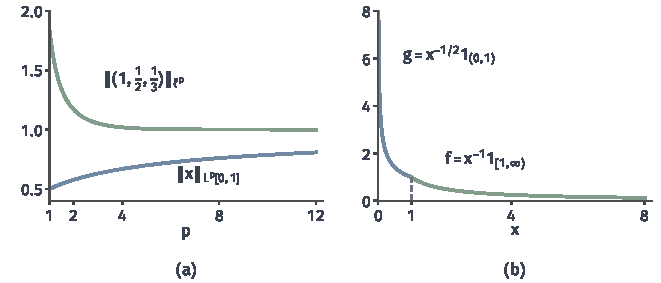
\includegraphics[width=112mm]{figures/04-spaces-measures-and-geometry/03-function-spaces/matplotlib/lop-lp-inclusion/figure.pdf}
  \caption{$L^p$范数随指数变化的方向由测度决定。(a)概率测度上$\lVert x\rVert_{L^p[0,1]}=(p+1)^{-1/p}$随$p$增大（蓝），计数测度上$(1,1/2,1/3)$的$\ell^p$范数随$p$减小（绿）。(b)$(0,\infty)$上两种失败：尖峰$g=x^{-1/2}\mathbf 1_{(0,1)}$在$L^1\setminus L^2$中（蓝），长尾$f=x^{-1}\mathbf 1_{[1,\infty)}$在$L^2\setminus L^1$中（绿）。}
  \label{fig:lop-lp-inclusion}
\end{BookInlineFigure}

\subsection{改变测度后的范数比较}
\label{sec:lop-change-of-measure}

在同一个可测空间上换一个测度，函数的$L^p$范数就要用新测度计算。设$h\geq0$可测，$\nu$由$\mathrm d\nu=h\,\mathrm d\mu$给出，即$\nu(E)=\int_Eh\,\mathrm d\mu$；第~\ref{chap:measure-densities}章把$h$称为$\nu$关于$\mu$的密度。

按向量的类比，这相当于给每个分量换一个权重$h(x)$。我们想知道$L^p(\mu)$中的误差能否控制$L^p(\nu)$中的误差，下面设$1\leq p<\infty$。

\paragraph{等价类的对应}
比较之前先要说明映射本身有意义。$L^p(\mu)$的元素是$\mu$几乎处处相等的等价类，$L^p(\nu)$的元素是$\nu$几乎处处相等的等价类。

若$f=g$在$\mu$几乎处处成立，记$N=\{f\neq g\}$，则$\mu(N)=0$，从而
\[
 \nu(N)=\int_Nh\,\mathrm d\mu=0.
\]
所以$\mu$等价类中的函数在$\nu$下也属于同一个等价类，映射$J[f]_\mu=[f]_\nu$不依赖代表的选取。这一步用的正是$\nu$关于$\mu$绝对连续：$\mu$零测集也是$\nu$零测集。

\begin{theorem}[有界密度给出有界映射]
\label{thm:lop-change-of-measure}
设$\mathrm d\nu=h\,\mathrm d\mu$，且存在常数$C$使$h\leq C$在$\mu$几乎处处成立。则对$f\in L^p(\mu)$有$f\in L^p(\nu)$，并且
\begin{equation}
 \lVert f\rVert_{L^p(\nu)}\leq C^{1/p}\lVert f\rVert_{L^p(\mu)} .
 \label{eq:lop-change-of-measure}
\end{equation}
所以$J:L^p(\mu)\to L^p(\nu)$是有界线性映射，$\lVert J\rVert\leq C^{1/p}$。
\end{theorem}

\begin{proof}
对非负可测函数$\lvert f\rvert^p$，由密度的定义，
\[
 \int\lvert f\rvert^p\,\mathrm d\nu=\int\lvert f\rvert^ph\,\mathrm d\mu\leq C\int\lvert f\rvert^p\,\mathrm d\mu.
\]
开$p$次方即得。线性由$J$在代表上作恒等变换得到。
\end{proof}

\paragraph{映射可能不是单射}
权重为零的分量不再被计入，所以$J$不一定区分$L^p(\mu)$中不同的元素。若$h=0$在某个满足$0<\mu(A)<\infty$的集合$A$上成立，则$\mathbf 1_A$在$L^p(\mu)$中非零，但
\[
 \int\mathbf 1_A\,\mathrm d\nu=\int_Ah\,\mathrm d\mu=0,
\]
所以$J\mathbf 1_A=0$。新测度看不见$A$上发生的事情，$\ker J$由在$\{h>0\}$上几乎处处为零的函数组成。

若$h>0$在$\mu$几乎处处成立，两种零测集就一致。一方面，绝对连续已给出由$\mu(E)=0$推出$\nu(E)=0$。另一方面，若$\nu(E)=\int_Eh\,\mathrm d\mu=0$，则$h\mathbf 1_E=0$在$\mu$几乎处处成立，而$h>0$几乎处处，只能$\mathbf 1_E=0$几乎处处，即$\mu(E)=0$。

这时两种等价类相同，$J$是单射；但$h$可以任意接近零，$J$仍可能不满射，逆映射也可能无界。在$[0,1]$上取$h(x)=x$，函数$x^{-3/4}$满足$\int x^{-3/2}\cdot x\,\mathrm dx<\infty$，属于$L^2(\nu)$，而$\int x^{-3/2}\,\mathrm dx=\infty$，不属于$L^2(\mu)$，所以$J$不是满射。

若密度还有正下界，即$0<c\leq h\leq C$几乎处处，同样的计算给出
\begin{equation}
 c^{1/p}\lVert f\rVert_{L^p(\mu)}\leq\lVert f\rVert_{L^p(\nu)}\leq C^{1/p}\lVert f\rVert_{L^p(\mu)} .
 \label{eq:lop-measure-equivalence}
\end{equation}
这时$L^p(\mu)$与$L^p(\nu)$是同一个函数空间，两个范数等价。例如在$[0,1]$上取$h(x)=1+x$，有$1\leq h\leq2$，两个$L^2$范数之比始终在$1$与$\sqrt2$之间。

若取$h(x)=x$，下界消失。令$f_n=\sqrt n\,\mathbf 1_{(0,1/n)}$，则$\lVert f_n\rVert_{L^2(\mu)}=1$，而
\[
 \lVert f_n\rVert_{L^2(\nu)}^2=n\int_0^{1/n}x\,\mathrm dx=\frac1{2n}\to0.
\]
反方向的控制不存在。权重越接近零的区域，越能藏住$\mu$意义下的大函数。
